\begin{enumerate}
    \item \textbf{As seen in Table \ref{tab:pre_lab_matching} the MOSFETs with different channel cases have differing gate to source voltages ($V_{GS}$) vs drain to source voltages. ($V_{DS}$). We also know that $V_T$ = 2.5 V}

\begin{table}[h]
    \begin{tabular}{@{}ccc@{}}
    \toprule
    \textbf{$V_{GS}$ (V)} & \textbf{$V_{DS}$ (V)} & \textbf{Refers to graph} \\ \midrule
    +2                    & 0.0                   & A                         \\
    +5                    & +5.0                  & E                         \\
    -1                    & +7.0                  & A                         \\
    +7                    & +1.0                  & C                         \\
    +5                    & 0.0                   & B                        \\
    +5                    & +4.0                  & D                         \\
    +7                    & +4.5                  & E                         \\
    +7                    & +5.0                  & F                         \\
    +3                    & 0.0                   & B                         \\
    +5                    & +2.5                  & B                         \\ \bottomrule
\end{tabular}
    \caption{Different voltages applied to an n-channel MOSFET}
    \label{tab:pre_lab_matching}
\end{table}

\begin{figure}[h]
    \centering
    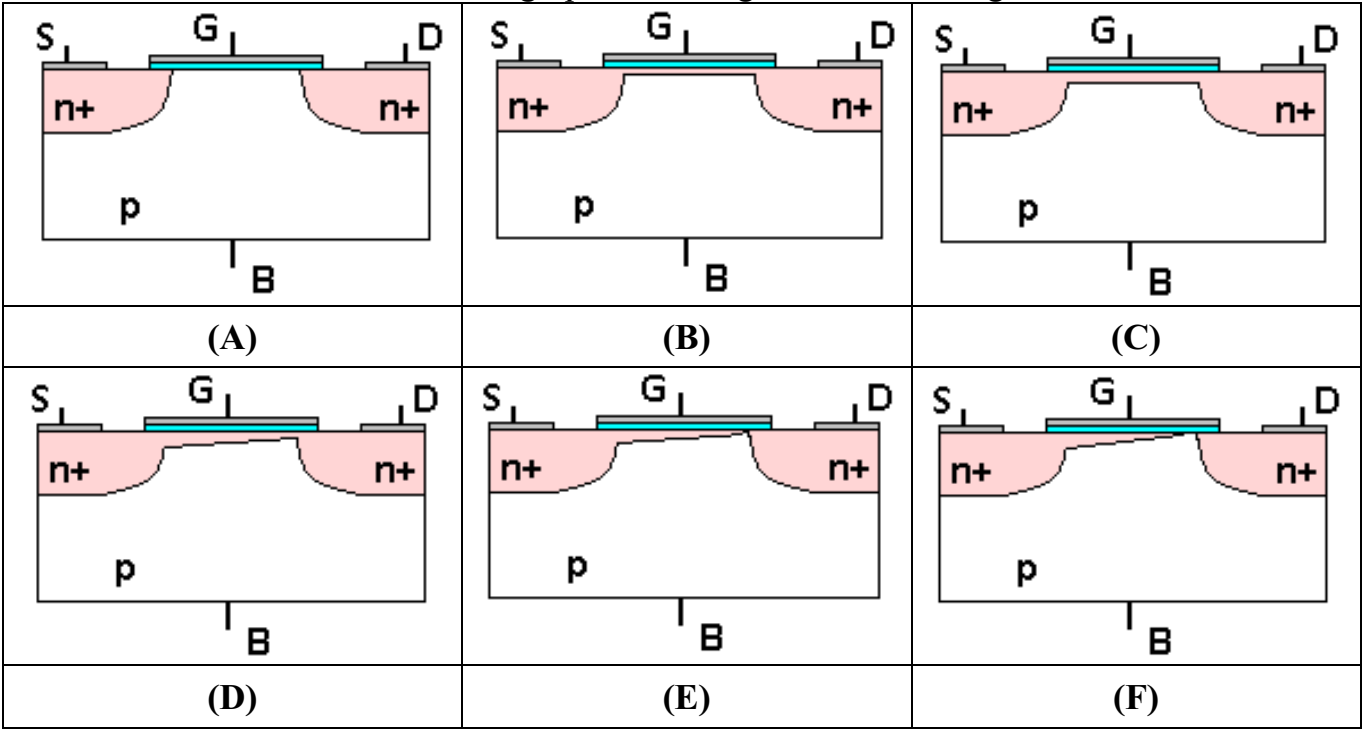
\includegraphics[width=.75\linewidth]{figures/prelab_MOSFETS.png}
    \caption{N-MOSFETs with different channel cases}
    \label{fig:prelab_MOSFETS}
\end{figure}

\clearpage

    \item \textbf{Operation of a n-channel enhancement MOSFET}

An n-type enhancement MOSFET is normally off when the gate-source voltage is 0 $(V_{GS}=0)$. However, if a voltage is applied to its gate lead, the drain-source channel becomes less resistive. To turn on a N-Channel Enhancement-type MOSFET, you need to apply a sufficient positive voltage $V_{DS}$ to the drain of the transistor as well as a sufficient positive voltage to the gate of the transistor. This allows a current to flow through the drain-source channel. With a sufficient positive voltage, $V_{DS}$, and sufficient positive voltage applied to the gate, the N-Channel Enhancement-type MOSFET is fully functional and is in the 'ON' operation. \\
Conversely to turn off an N-channel Enhancement MOSFET, you can either cut off the bias positive voltage, $V_{DS}$, that powers the drain. Or you can turn off the positive voltage going to the gate of the transistor
\begin{figure}[ht] 
  \begin{subfigure}[b]{0.40\linewidth}
    \centering
    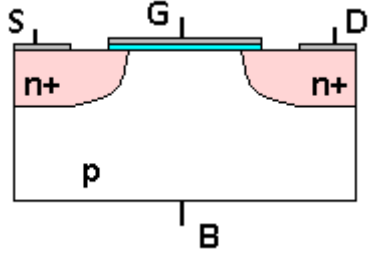
\includegraphics[width=0.90\linewidth]{figures/prelab_no_flow.png} 
    \caption{Below Threshold, $V_{GS} < V_T$ \& $V_{DS}>$ 0}
    \label{fig:no_flow} 
    \vspace{4ex}
  \end{subfigure}
  \begin{subfigure}[b]{0.40\linewidth}
    \centering
    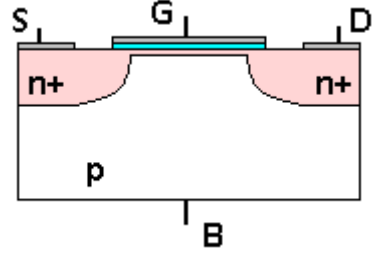
\includegraphics[width=0.90\linewidth]{figures/prelabb_channel.png} 
    \caption{Above Threshold} 
    \label{fig:channel} 
    \vspace{4ex}
  \end{subfigure}\\
  \begin{subfigure}[b]{0.40\linewidth}
    \centering
    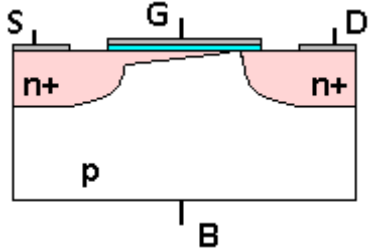
\includegraphics[width=0.90\linewidth]{figures/prelab_pinched.png} 
    \caption{Above Threshold} 
    \label{fig:pinched} 
    \vspace{4ex}
  \end{subfigure}
  \caption{}
  \label{fig:nMOS} 
\end{figure}
\end{enumerate}
